\documentclass{article}[12pt]

\usepackage{amsmath}
\usepackage{graphicx}
\usepackage{float}
\usepackage{xcolor}
\usepackage{listings}
\usepackage{url}
\usepackage{amsmath}
\usepackage{geometry}
\usepackage{tcolorbox}
\usepackage{amssymb}
\usepackage{url}
 \geometry{
 a4paper,
 total={170mm,257mm},
 left=20mm,
 top=20mm,
 }
 

 
 \definecolor{mGreen}{rgb}{0,0.6,0}
\definecolor{mGray}{rgb}{0.5,0.5,0.5}
\definecolor{mPurple}{rgb}{0.58,0,0.82}
\definecolor{backgroundColour}{rgb}{0.95,0.95,0.92}

\lstdefinestyle{CStyle}{
    backgroundcolor=\color{backgroundColour},   
    commentstyle=\color{mGreen},
    keywordstyle=\color{magenta},
    numberstyle=\tiny\color{mGray},
    stringstyle=\color{mPurple},
    basicstyle=\footnotesize,
    breakatwhitespace=false,         
    breaklines=true,                 
    captionpos=b,                    
    keepspaces=true,                 
    numbers=left,                    
    numbersep=5pt,                  
    showspaces=false,                
    showstringspaces=false,
    showtabs=false,                  
    tabsize=2,
    language=C
}

\begin{document}

 \setlength\parindent{0pt}

\begin{center}
\huge{\textbf{CTmeasure\\Contactless Temperature Measurement}}
\end{center}

\begin{center}
\textbf{Author: nmt@nt-com.org}
\end{center}

\abstract{This document describes the CTmeasure project on the STM32F401RE and the 8-bit ATMega328p microcontroller. With the proof of concept working on the STM32 platform, the next step is porting the project to a smaller controller. As I only have a ATMega328p at my disposal, I chose this microcontroller for the next step in the project. Again, \textbf{THIS IS NOT A MEDICAL DEVICE, I AM NOT A MEDICAL PROFESSIONAL.} The aim of this project is to implement contactless temperature measurement using appropriate IR sensors and to display the data on a computer.}

\section{Introduction}

\subsection{Motivation}

The recent COVID-19 infections demand measures regarding the detection of infected individuals to help combat the spread of the virus. Recently the media has reported of instances around the globe where fever is measured in front of public buildings (for instance supermarkets). After registering with the group "HelpfulEngineering" on Slack and reading the contributions of members, I started working on a way to measure temperatures without contact using infrared technology. The credit belongs to these groups, I am merely supporting their effort.

\subsection{Method}

The core of this project is the MLX90614 temperature sensor in the BAA version. This sensor measures temperatures using infrared technology without being in contact with the measured object. The $I^2C$ bus is used to interface between the sensor and a microcontroller. Next, the measured data must be converted to human-readable form and be displayed in some way. I chose to send the data to a PC and display it there. This is accomplished by the microcontrollers USART peripheral. I do not use any HALs or APIs with this project, everything is programmed from the ground up.

\section{ATMega328p Software}

\subsection{Software Modules Microcontroller}

The software consists of three main parts: 

\begin{enumerate}
	\item The drivers (UART, I2C, 16-bit Timer)
	\item The interfacing to the MLX90614 sensor
	\item The application itself carrying out the timed measurements
\end{enumerate}

The inline documentation of the code is extensive and references all parts of the ATMega328p datasheet needed to understand it. Further, relevant formula are explained in the inline documentation. An overview of the interfaces is given in the header files, details explained in the c files. The files included are:

\begin{itemize}
	\item twi.h twi.c (I2C interfacing)
	\item uart.h uart.c uart\_cfg.h (UART interfacing)
	\item tim16.h tim16.c tim16\_cfg.h (16-bit timer)
	\item debug.h debug.c debug\_cfg.h (debugging helpers)
	\item mlx90614.c mlx90614.h (sensor interfacing)
	\item main.c 
\end{itemize}

\subsection{Program Flow}

The software does an initialization of all the microcontroller peripherals in the main.c file in a first step. This includes the UART, I2C and the 16-bit timer. After that the software enters the superloop (while(1)). The measurements and the subsequent data transmission to the PC are done in an interrupt service routine (ISR). This ISR is triggered every 200ms. That means five measurements are done per second and the results are transmitted to the PC. This is depicted in fig. \ref{fig:swflow}.


\begin{figure}[H]
  \caption{Flow of the Microcontroller Program.}
  \label{fig:swflow}
  \centering
    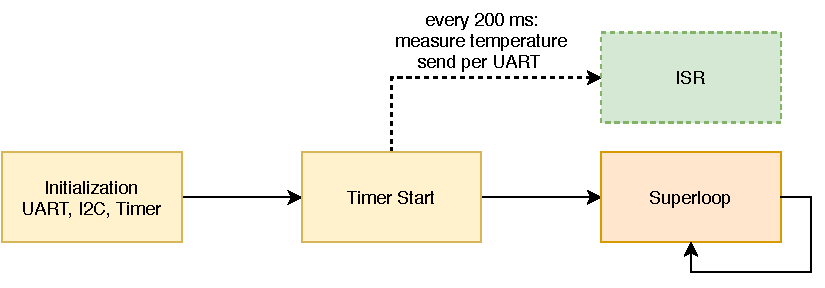
\includegraphics[width=0.75\textwidth]{img/swflow.pdf}
\end{figure}

A major chance is that instead of doing the expensive floating point calculations on the microcontroller, only the raw sensor data is sent to the PC. Here, the UI must do the necessary calculations to convert the raw sensor values to a human readable temperature. 

\subsection{Debugging the Microcontroller Code}

In order to be able to debug the microcontroller code, I added debugging functionality. There are two main parts to the debugging module. First, debugging is turned on an off in the file debug\_cfg.h. When debugging is on an LED connected to pin D6 of the microcontroller is initialized. This LED is off until the timer ISR starts, where it is toggled each time the ISR is executed. Further, error codes, if there are any errors, are transmitted through the UART. See the inline documentation for details. What I will mention here is that information about the initialization routines is sent when debugging is activated, as well as information about each step of the I2C process (if there are errors).

I use preprocessor flags to activate/deactivate the debugging. This makes the code a little hard to read, but is worth a lot when problems are encountered. One note here: The routine to interface with the MLX90614 always returns a status code. When debugging is off, this return value is simply ignored in the software in the current state.

\section{STM32F401RE Software}

As a microcontroller I chose the STM32F401RE, which I had available as a prototyping platform. Here, I coded some of the drivers through a course I did a while back and the missing parts by myself. The code does not use any HAL or API, it is written from the ground up to remove all unnecessary parts, hopefully resulting in a small codebase with minimal complexity.

In order to display the measured data on a PC, I connect the bluetooth module as a serial port. Through a python script utilizing the serial and matplotlib library I am able to plot the data in "real-time".

To get an overview of the software, refer to fig. \ref{fig:swflow.pdf} in the previous section. As both the STM32F401RE and ATMega328p software work in the same way and are only organized differently, I will omit an explanation of the STM32 software. It is extensively documented in the code and the documentation in the previous section establishes the concrete workings of the software.

The key difference in both software versions is the use of the bluetooth module with the STM32 platform, the ATMega328p platform does feature the bluetooth option.

\section{Hardware}

\subsection{ATMega328p Version}

As a test platform I am using a cheap Arduino Nano clone, I have nothing else at my disposal. This has consequences for the project. First, I can't add the UART bluetooth module as I did in the proof of concept, the UART is already used on this board. I know that there is an Arduino software serial library to get around this, but I don't want to use a bit-banged UART (concerns about stability and speeds). Thus, the bluetooth module is gone, instead I am connecting per cable to the Nano to get the temperature values per serial interface.

As far as I2C is concerned, no external pullups are needed. The sensor features $10k\Omega$ pullups. The sensor is powered via the board's $3.3V$ output. The only other (not strictly necessary component) is the debug LED that does not need to be included and is deactivated once debugging mode is turned off. The complete setup is shown in fig. \ref{fig:hwsetup}. If a custom board would be made, the UART could be used for a bluetooth module as in the proof of concept. The only change in the software would be, if necessary, a different UART baudrate.

\begin{figure}[H]
  \caption{Hardware Setup for the Arduino Nano.}
  \label{fig:hwsetup}
  \centering
    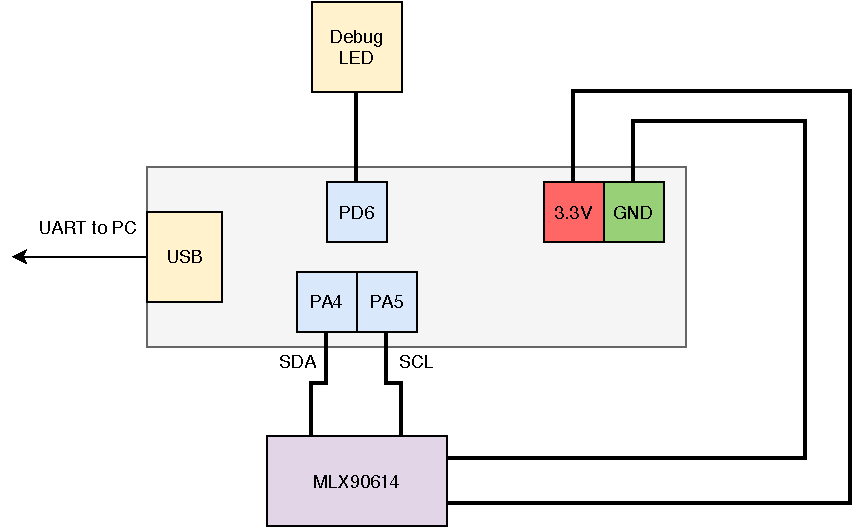
\includegraphics[width=0.75\textwidth]{img/hwsetup.pdf}
\end{figure}

\subsection{STM32 Version}

An overview of the hardware setup is depicted in fig. \ref{fig:stm32hw}. I chose to provide a simplified version of the schematics of the Nucleo Board, showing the connection of each peripheral. 

\begin{figure}[H]
  \caption{Hardware Setup for the STM32F401 Nucleo Board.}
  \label{fig:stm32hw}
  \centering
    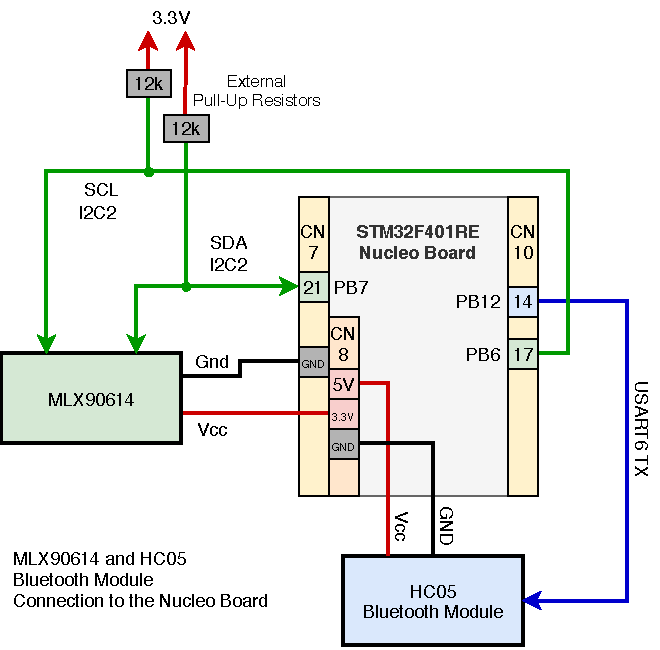
\includegraphics[width=0.75\textwidth]{img/stm32_block.pdf}
\end{figure}

There is one main pitfall, described in the following:

\begin{enumerate}
\item The internal pull-ups of the STM32F4 ARE NOT SUFFICIENT! Use external pull-ups, currently I am using 12kOhms. 
\item The MLX90614 demands a repeated start condition after the register that shall be read is communicated to the sensor
\end{enumerate}

If (1) is not considered, the I2C timing requirements are violated, making repeated start impossible (2), thus the sensor does not respond with any data. This is solved in my code and the hardware setup. 

\section{User Interface}

The user interface is a hacked together mess and I am confident it could be done much better by someone with more experience in this area. However, it does it's job and that is to show the temperature currently being measured. In this new design iteration of the project, there are two interfacing scripts, both written in python. 

One script shows the sensor values as floating point numbers when started and has no graphical output. The graphical output script is pretty much the same as in the proof of concept, with two modifications: 

\begin{enumerate}
	\item The raw temperature value must be converted to a floating point value, as with the script showing the raw values.
	\item During the time temperature is measured, the mean value of all temperatures currently in the measurement window is calculated and displayed.
\end{enumerate}

The second point gets rid of any peaks and bumps and so on in a simple manner, providing the user of the project with a more stable temperature output. However, this only a quick, simple fix one can do. Maybe there is a better way to get a smooth output. 

An example of this is shown in fig. \ref{fig:ambienttemp} showing an ambient temperature measurement. The green dots are samples taken in $200ms$ intervals, the red line shows the average temperature over the measurement window. I can confirm the accuracy through an analog thermometer (more or less as it is analog).

\begin{figure}[H]
  \caption{Ambient Temperature Measurement.}
  \label{fig:ambienttemp}
  \centering
    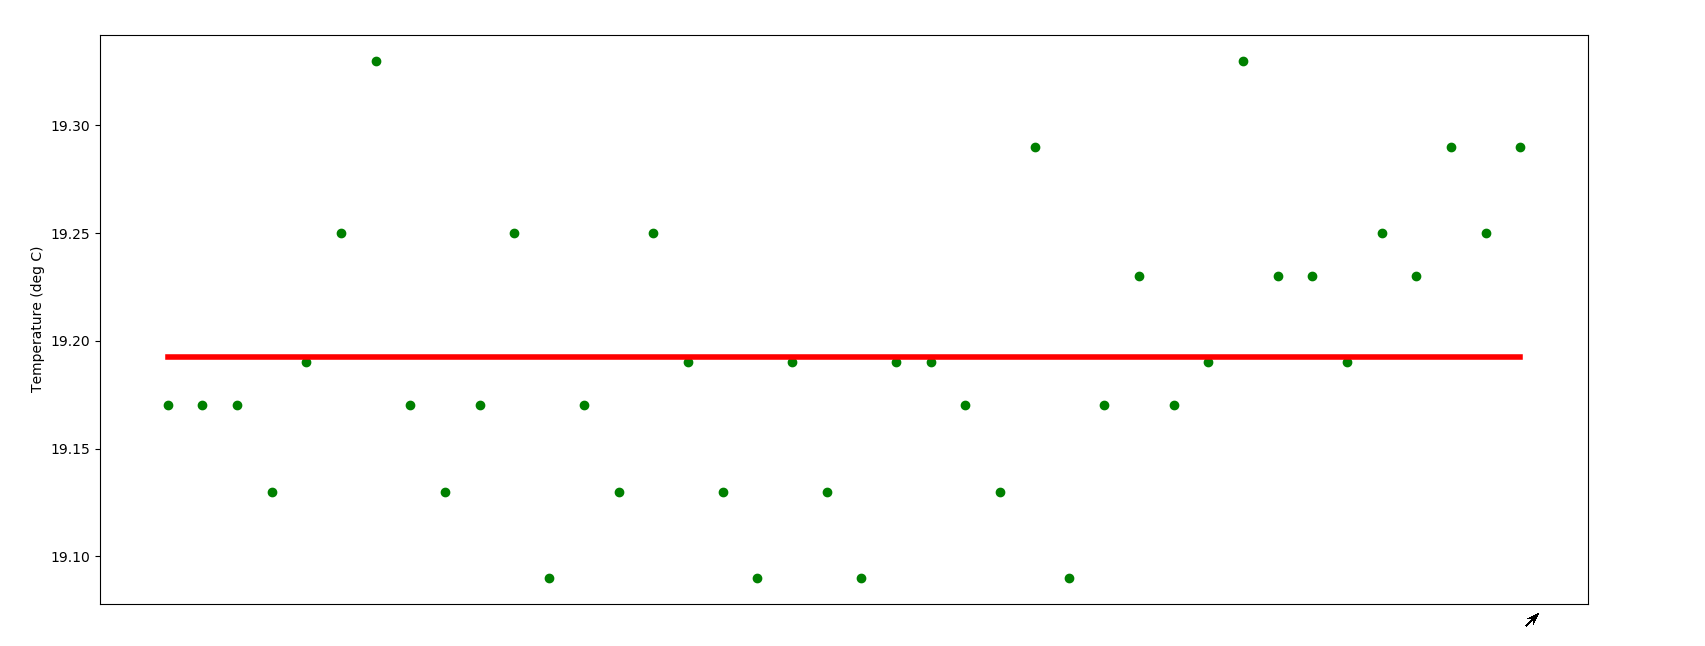
\includegraphics[width=0.75\textwidth]{img/ambienttemp.png}
\end{figure}

The next measurement is again a forehead measurement, depicted in fig. \ref{fig:foreheadtemp1}. Here, I measured for approximately $30$ seconds, with a distance of about 1-2 centimeters to the sensor.

\begin{figure}[H]
  \caption{Forehead Temperature Measurement 1.}
  \label{fig:foreheadtemp1}
  \centering
    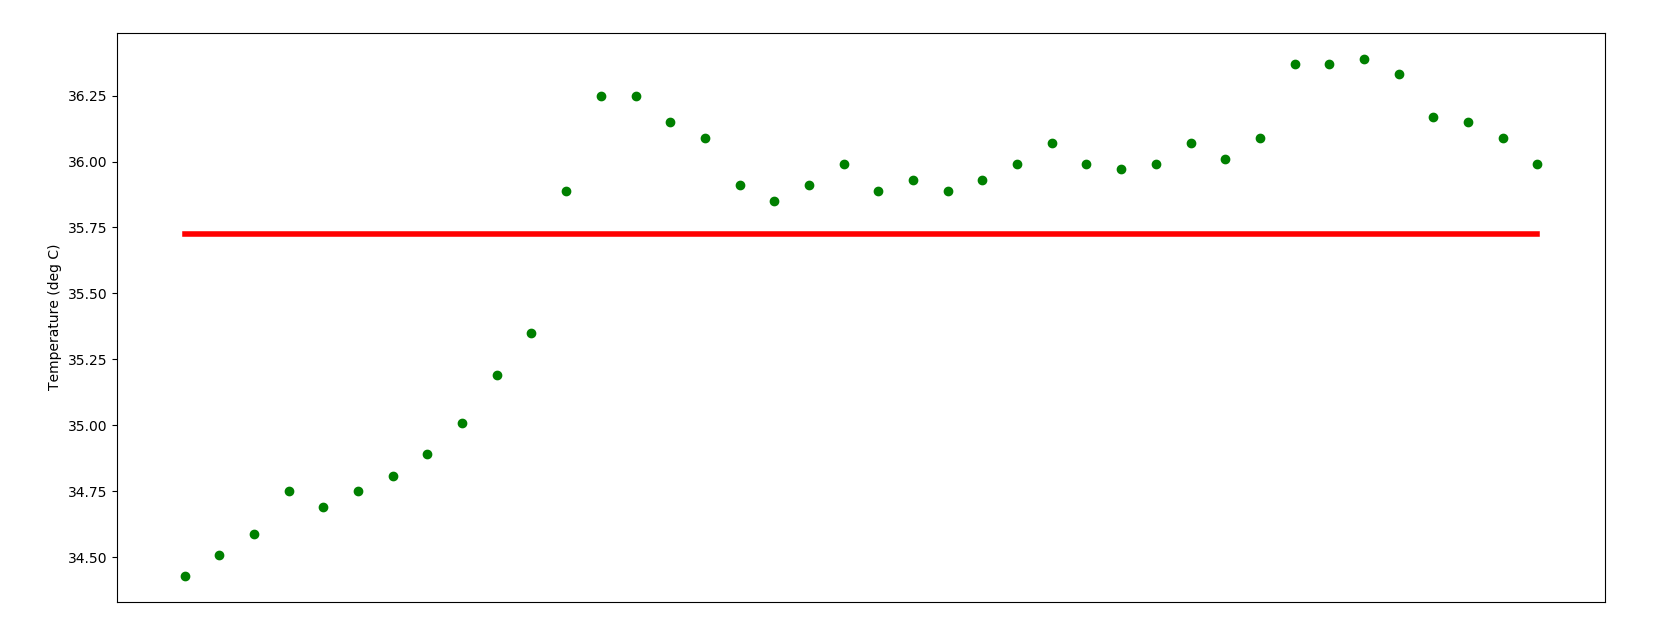
\includegraphics[width=0.75\textwidth]{img/foreheadtemp1.png}
\end{figure}

In fig. \ref{fig:foreheadtemp2} you can see that the measurement stabilizes after about $30-40$ seconds. 

\begin{figure}[H]
  \caption{Forehead Temperature Measurement 2.}
  \label{fig:foreheadtemp2}
  \centering
    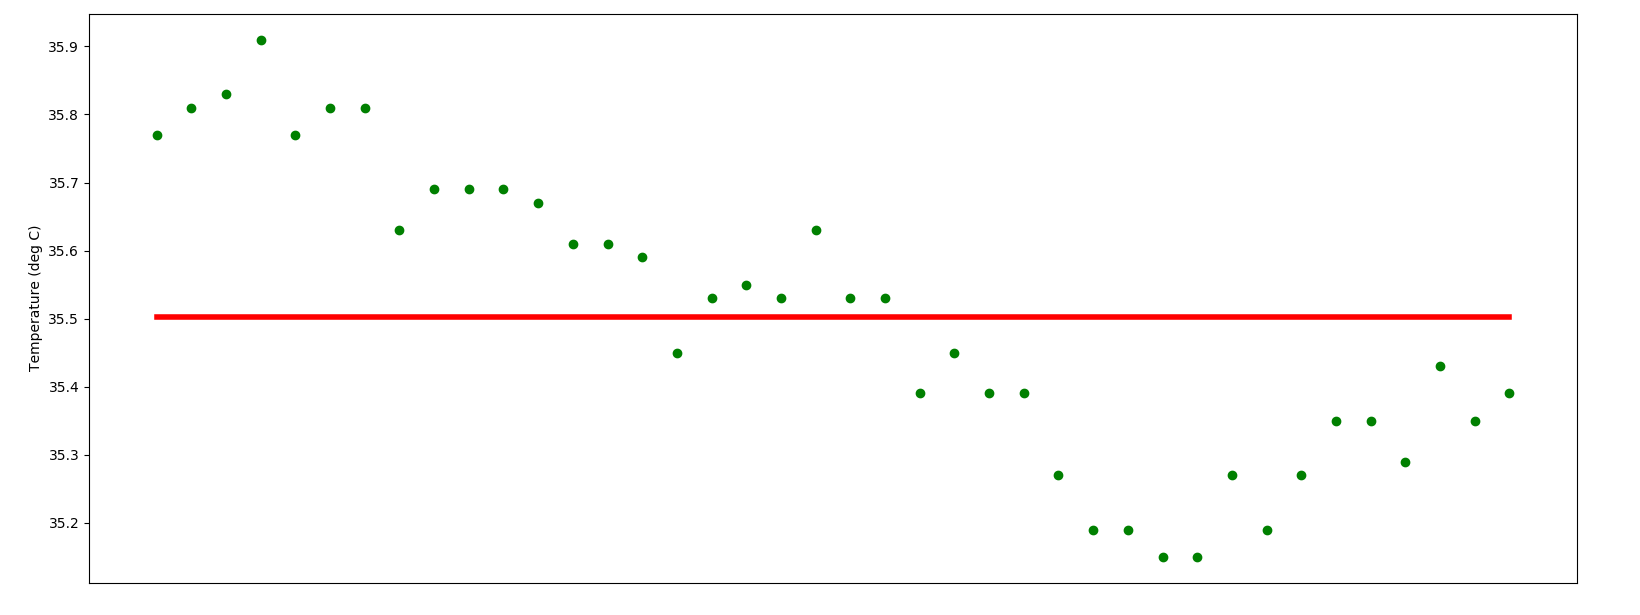
\includegraphics[width=0.75\textwidth]{img/foreheadtemp2.png}
\end{figure}

The above measurements were carried out on the Arduino platform. There is a slight difference between the measurements carried out by the ATMega328p and the STM32. The Arduino sends the raw temperature values to the PC, which converts them to float format. The STM32 platform does the floating point conversion directly after measurement and sends to floating point value to the PC as a string.

\subsection*{Problems with this Approach}

Plotting the data in "real-time" results in some problems regarding stabilization time $t_st$. When using the graphical output of the UI, a lag makes $t_s$ seem to be about $30s$. However, this is not the case in reality. From various measurements using the script WITHOUT graphical output I can confirm a short stabilization time when doing temperature measurements. To detect a change in temperature, it takes about $0.5$ to $1s$. Thus, the plotting of the data in this manner makes $t_s$ seem much larger than it actually is. The graphical output in the provided form can be used for debugging and visualization, however for practical use it is, in my opinion, not an optimal solution and should be reworked. 

\section{Conclusion}

From measurements and discussions with the group the main pitfall in this project turns out the be the MLX90614 in the BAA version. Because of its field of view, the user must be very close (I measured 0.5-1.0cm) to the sensor for an accurate measurement. However, alternative versions of the MLX90614 exist that may mitigate this problem. For further info please refer to: \url{https://github.com/helpfulengineering/project-temperature-detection}. All in all, the software in the current state is documented and tested. As it works as intended, changing the particular sensor does not require changes to the software as far as I can see. 

\section{Future Work}

There are various future improvements. The software should incorporate further debugging capabilities, for easier use. Further, a display could be added directly to the microcontroller, thus a PC to display the data is no longer needed. As the ESP32 platform is very popular and widely available, the software could also be ported for use with the ESP32 boards. 





\end{document}